
\chapter{Monte Carlo Generation}  

\noindent You can visit the Overleaf Documentation library at: https://www.overleaf.com/learn or the official \LaTeX\ wiki at: \textbf{https://en.wikibooks.org/wiki/LaTeX} for in-depth guides to the \LaTeX\ typesetting system.

\section{How to incorporate citations in your document}


\noindent Make sure you have your references file in \textbf{.bib format}. You can export it from Mendeley and copy/paste them into the \textbf{referencias bib} file. Using the \textbf{citecommand}, start writing your source identifier and Overleaf will automatically show you the available references. A sample citation \cite{dirac}. If you want to cite two references \cite{einstein,knuth-fa} or \cite{einstein},\cite{knuth-fa}. Citing a range of references \cite{einstein,knuth-fa,radiation2}.


\subsection{Citation Styles}
\noindent There are several bibliography styles to choose from: \textbf{abbrv, acm, alpha, apalike, ieeetr, plain, siam, unsrt.} The default is ieeetr. Remember to change the option in the document preamble in \textbf{tesis.tex} %WRITE HERE


\section{Using Images}




%FIGURE  EXAMPLES___________________________________________________________________________

\noindent This is an example of a figure, as shown in Figure \ref{gric}. Your images must be uploaded to the \textbf{images} folder. Accepted file formats are \textbf{pdf, png, jpg, and eps}. Use the following options for the location of the image on the page: \textbf{[htbp]} that refer to here, top, bottom, or special page. Pay attention to the image width. If the image is wider than the margins, \LaTeX\ will produce an warning or error.

\begin{figure}[h]
\begin{center}
\includegraphics[width=0.3\textwidth]{images/GRIC} %specify width
\end{center}
\caption{GRIC logo!!} %specify caption
\label{gric}
\end{figure}

%


\subsection{Adding Subfigures}
\noindent If you need to place two subfigures in your figure, follow the example below:

\begin{figure}[h!]
\begin{subfigure}{.48\textwidth}
  \centering
  % include first image
  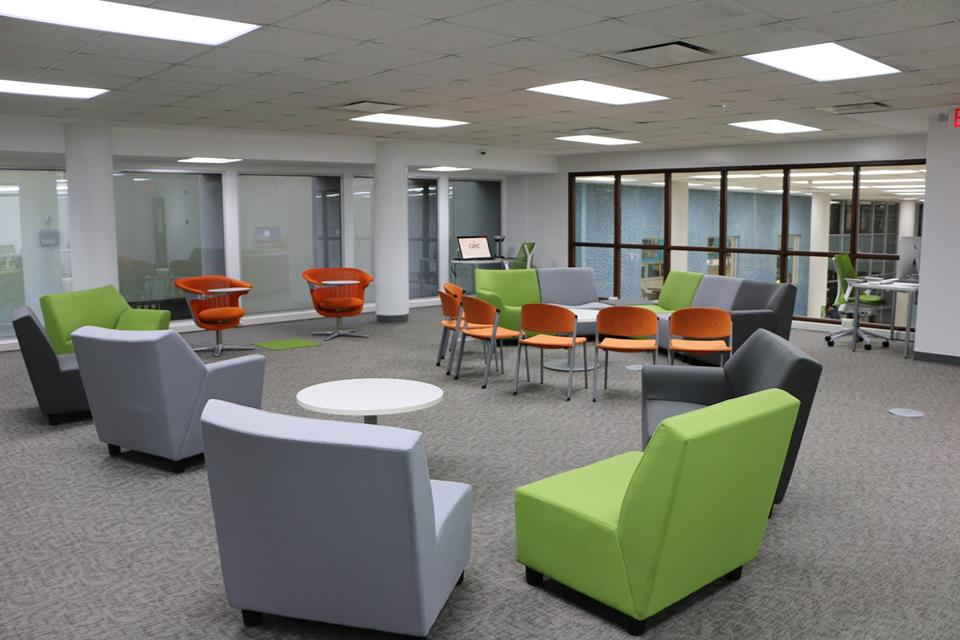
\includegraphics[width=.8\linewidth]{images/2}  
  \caption{Put your sub-caption here}
  \label{fig:sub-first}
\end{subfigure}
\begin{subfigure}{.48\textwidth}
  \centering
  % include second image
  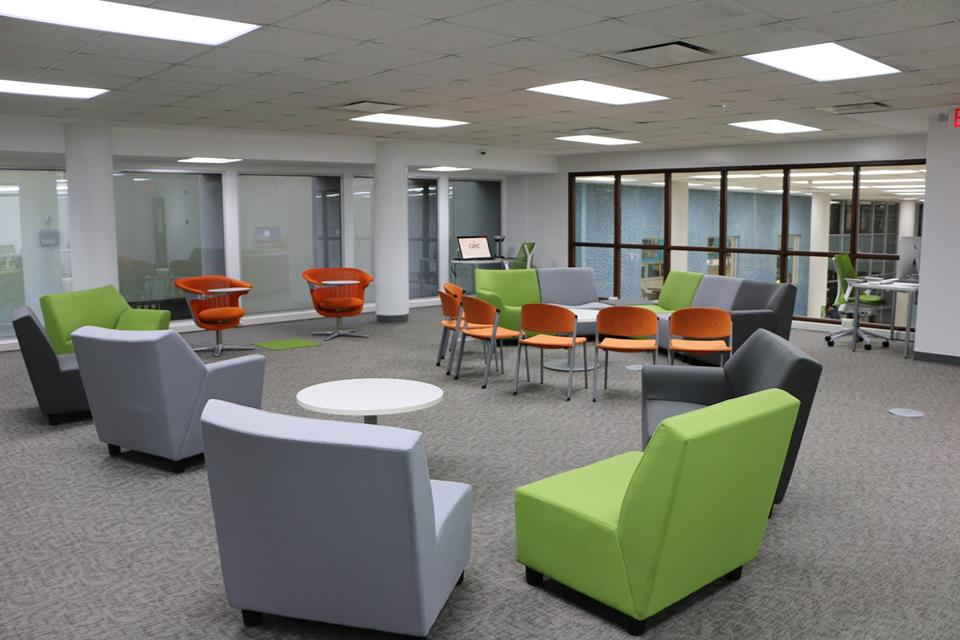
\includegraphics[width=.8\linewidth]{images/2}  
  \caption{Put your sub-caption here}
  \label{fig:sub-second}
\end{subfigure}
\caption{Put your caption here}
\end{figure}


\noindent If you need to place four subfigures in your figure, follow the example below, but \LaTeX\ is very particular with widths, so you have to play around with the numbers.It might give you overflow warnings. These won't stop your document from compiling.  It is easier to build the four images as a single one before uploading it to Overleaf.

\begin{figure}[ht]
\begin{subfigure}{.5\textwidth}
  \centering
  % include first image
  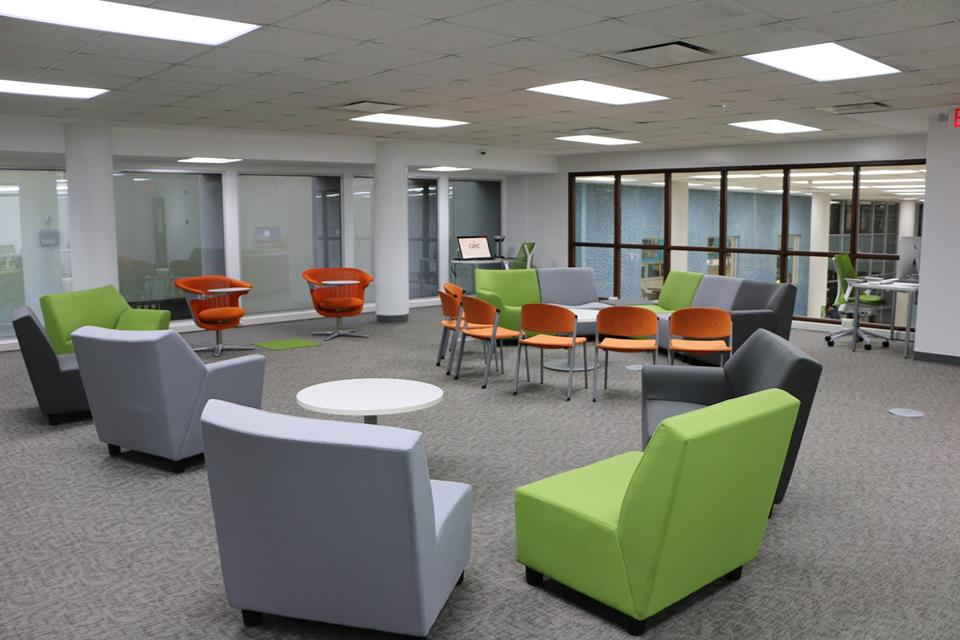
\includegraphics[width=.8\linewidth]{images/2}  
  \caption{Put your sub-caption here}
  \label{fig:sub-firstfirst}
\end{subfigure}
\begin{subfigure}{.5\textwidth}
  \centering
  % include second image
  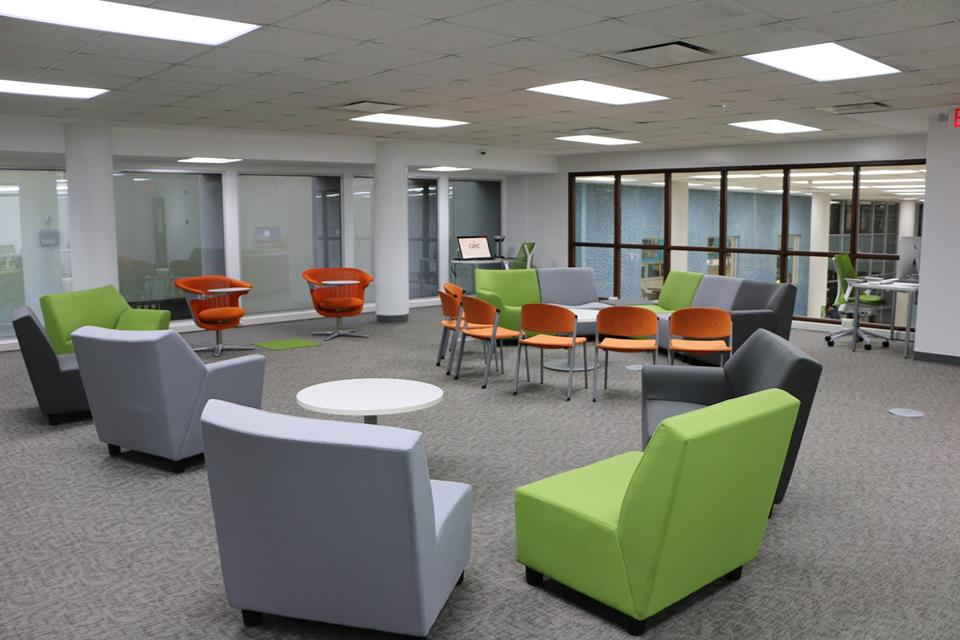
\includegraphics[width=.8\linewidth]{images/2}  
  \caption{Put your sub-caption here}
  \label{fig:sub-secondsecond}
\end{subfigure}
\begin{subfigure}{.5\textwidth}
  \centering
  % include third image
  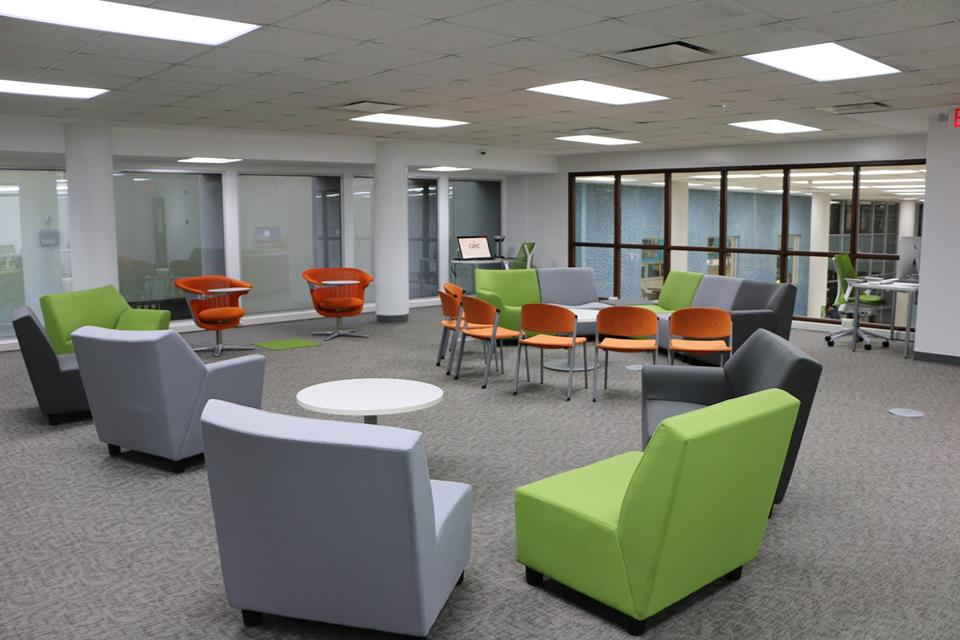
\includegraphics[width=.8\linewidth]{images/2}  
  \caption{Put your sub-caption here}
  \label{fig:sub-thirdthird}
\end{subfigure}
\begin{subfigure}{.5\textwidth}
  \centering
  % include fourth image
  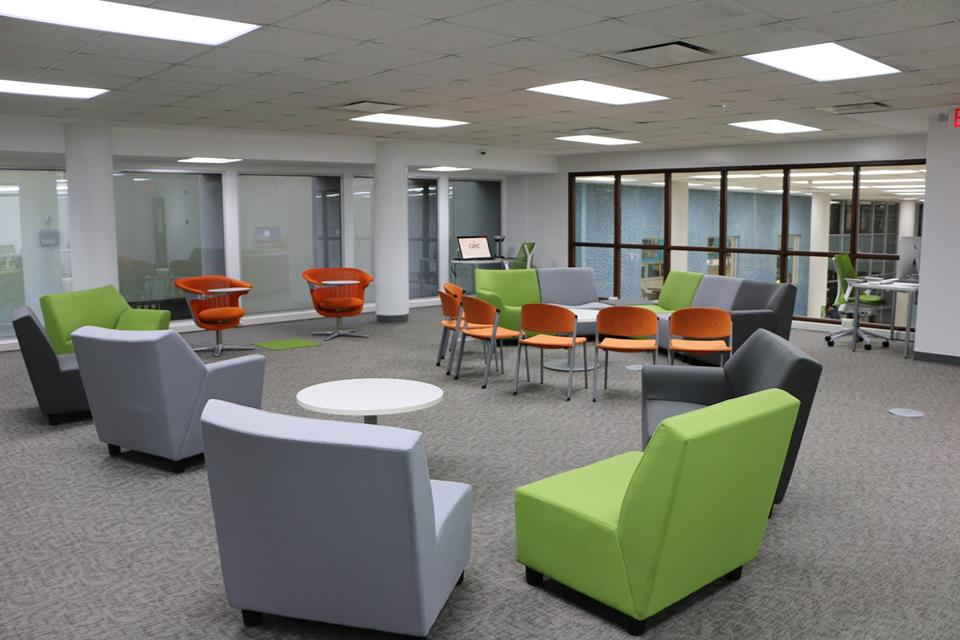
\includegraphics[width=.8\linewidth]{images/2}  
  \caption{Put your sub-caption here}
  \label{fig:sub-fourthfourth}
\end{subfigure}
\caption{Put your caption here}
\label{fig:fig}
\end{figure}

\section{Plotting Graphs}

\noindent You can import graphs as images, but you can also plot graphs in \LaTeX\ using pgfplots. This is a visualization tool to make it simpler to include plots in your documents. The basic idea is that you provide the input data/formula and pgfplots does the rest. You are welcome to experiment with this package, but really, but please, just use excel and export the image! A sample graph is shown in Figures \ref{fig:my_label} and \ref{fig:my_label2}. For additional examples, go to: \textbf{http://pgfplots.sourceforge.net/gallery.html}.

\begin{figure}[!ht]
    \centering
    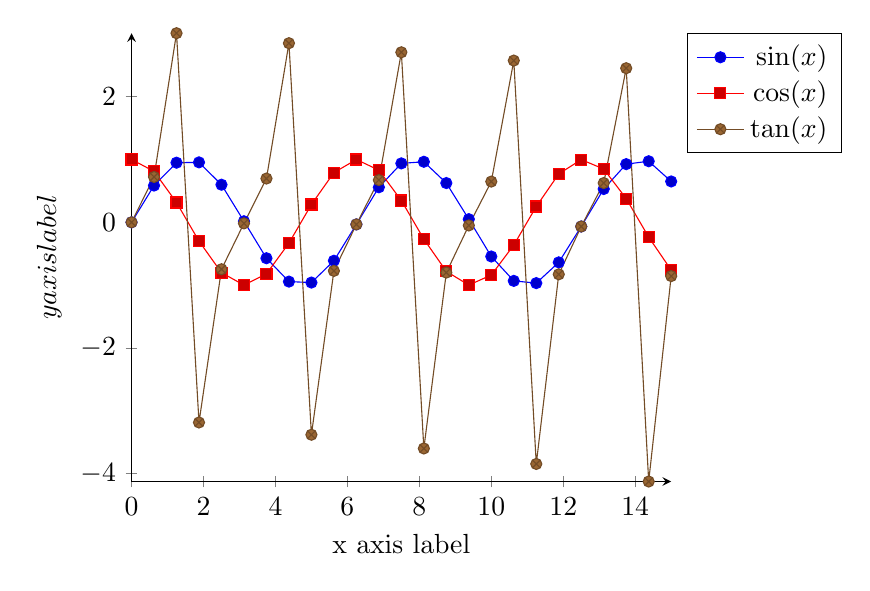
\begin{tikzpicture}
        \begin{axis}[domain=0:15,axis lines = left,
            xlabel = x axis label, %para texto
            ylabel = {\(y axis label\)}, %para notacion matematica
            legend style={cells={anchor=east},legend pos=outer north east}
	]
        \addplot {sin(deg(x))}; 
        \addplot {cos(deg(x))}; 
        \addplot {tan(deg(x))}; 
        \legend{$\sin(x)$,$\cos(x)$,$\tan(x)$}
        \end{axis}
    \end{tikzpicture}
    \caption{Put your Caption}
    \label{fig:my_label}
\end{figure}

\begin{figure}[!ht]
    \centering
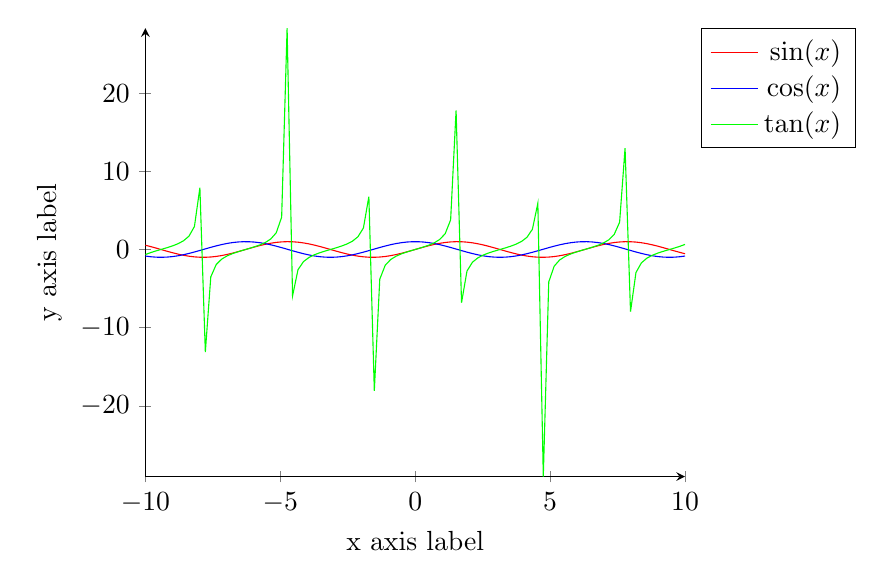
\begin{tikzpicture}
\begin{axis}[
    axis lines = left,
    xlabel = x axis label,
    ylabel = y axis label,
    legend style={
		cells={anchor=east},
		legend pos=outer north east}
]
%Plot1
\addplot [
    domain=-10:10, 
    samples=100, 
    color=red,
]
{sin(deg(x))};

%Plot2
\addplot [
    domain=-10:10, 
    samples=100, 
    color=blue,
    ]
{cos(deg(x))};

%plot3
\addplot [
    domain=-10:10, 
    samples=100, 
    color=green,
]
{tan(deg(x))};

%legend
\legend{$\sin(x)$,$\cos(x)$,$\tan(x)$}
legend pos=outer north east

\end{axis}
\end{tikzpicture}
\caption{Put another Caption}
    \label{fig:my_label2}
\end{figure}


%EQUATION EXAMPLES___________________________________________________________________________
\newpage
\section{Typing Equations in \LaTeX}

\noindent Writing equations is a bit complicated at first. It will become second nature once you get used to the symbols used. Equations are written between \textbf{begin equation and end equation} commands, and are referenced using theref command and the equation label, as in equation \ref{int1}:

\begin{equation}
\label{int1}
\int_{0}^{5}{\frac{2}{3}x}\ dx
\end{equation}

\noindent  You have several options for incorporating your equations in \LaTeX\ if you don't want to type them in the editor. Equation \ref{int1} was typed in MS Word Equation Editor and copied/pasted here. You can also use online equation converter tools, such as: \newline
 https://www.hostmath.com or https://latex.codecogs.com/eqneditor/editor.php.

\begin{equation}
\label{frac}
\frac{-b\pm\sqrt{b^2-4ac}}{2a}
\end{equation}


\begin{equation}
\label{int2}
\int_{0}^{\infty}x^{2}\ dx
\end{equation}



\subsection{Subsection}
\noindent \lipsum[1][1-3] %WRITE HERE

\subsection{Subsection}

\noindent \lipsum[1][4-6] %WRITE HERE